%\documentclass[journal]{IEEEtran}
\documentclass{report}
%\documentclass{ActaOulu}


\usepackage{amsmath}

\usepackage{graphicx}

\usepackage{amsfonts}

\begin{document}

\title{Artificial Intelligence}

\author{Jacopo Orlandini, 286416}

\maketitle

\begin{abstract}

Artificial intelligence (AI) has recently undergone a renaissance, making important progress in key areas such as control and decision making. This has been due, in part, to a large amount of available and cheap data and cheap compute resources, which have fit the natural strengths of deep
learning. In recent years, the quantity of information generated by business, government, and science has increase immensely - a phenomenon known as the \textit{data deluge}.
In parallel to this significant growth, data are also becoming increasingly interconnected. Facebook, for instance, is a graph nearly fully connected with 99.91 percent of individuals on the social network belonging to a single, large connected component.
Currently, most social networks connect people or groups who expose similar interests or features. More importantly, the interactions among people have significantly developed new frontiers in data science.
In this project I dive into citation network. Citation network is a social network which contains paper resources and linked by co-citation relationship (also called citation graph).
Recent advancements in deep neural networks for graph-structured data have led to state-of-the-art performance on graph convolutional network and node embedding.
Deep learning methods have an increasingly critical role in recommender
system applications, being used to learn useful lowdimensional
embeddings of text and individual users. The representations learned using deep models can be used to enhance performance in a graph convolutional neural network, and these learned representations
have high utility because they can be re-used in various tasks. For example, node embeddings can be used for citation recommendation.
Recent years have seen significant developments in this space—
especially the development of new deep learning methods that are
capable of learning on graph-structured data, which is fundamental
for recommendation applications.

\end{abstract}


\chapter{Introduction}

\section{Artificial Intelligence}
\textit{In which we describe agents can improve their behaviour through diligent study of their own experiences.}
\vspace{0.3cm}

In artificial intelligence, an intelligent agent is an autonomous entity which observes through sensors and acts upon an environment using actuators and directs its activity towards achieving goals. Intelligent agents may also learn or use knowledge to achieve their goals \cite{agent}. An agent is learning if it improves its performance on future tasks after making observations about its environment. In our case the agent is a  artifact able to take a graph as input and producing inference pattern between nodes.
Learning has the advantage that it allows the agents to initially operate in unknown environments and to become more competent than its initial knowledge alone might allow. The most important distinction is between the "learning element", which is responsible for making improvements, and the "performance element", which is responsible for selecting external actions.
A simple agent program can be defined mathematically as an function f (called \textit{agent function}) which maps every possible percepts sequence to a possible action the agent can perform or to a coefficient, feedback element, function or constant that affects eventual actions.
\begin{equation}
f:P^* \rightarrow A
\end{equation}

There are three major types of learning:

 In\textit{ unsupervised learning }the agent learn patterns in the input even though no explicit feedback is supplied. Clustering is the task of grouping a set of objects into groups based on the similarity of their features. Clustering belongs to exploration problems, where there is no knowledge about the state of the world. In \textit{reinforcement learning} the agent learns from a series of reinforcements-rewards or punishment. Reinforcement learning is an area of machine learning concerned with how software agents ought to take actions in an environment so as to maximize some notion of cumulative reward but requires clever exploration mechanisms. In \textit{supervised learning }, the agent observes some example input-output pairs and learns a function that maps input to output. In real world and real application, we can relax some constraints and create subset of these methods.
\section{Semi-Supervised Learning}
In semi-supervised learning we are given a few labeled examples and must make what we can of a large collection of unlabeled examples. Even the labels themselves may not be the oracular truths that we hope for. Thus, both noise and absence of labels create a continuum between supervised and unsupervised learning.
The task of supervised learning is this: 
given a training set of N example input-output pairs
\[(x_1,y_1), (x_2,y_2),...(x_N,y_N)\] where $y_i$ was generated by an unknown relation \[y_i = f(x_i),\] discover a function \[h\cong f\] that approximates \textit{f}.
To measure the accuracy of a hypothesis we give it a \textit{test set} of examples that are distinct from the training set. We say a hypothesis generalizes well if it correctly predicts the value of y for new examples. Sometimes the \textit{f} is stochastic, and we have to learn a conditional probability distribution.
When the output y is one of a finite set of values, we call the learning problem \textit{classification}. When y is a number, the learning problem is called \textit{regression}.

\begin{figure}[htbp]
\centering
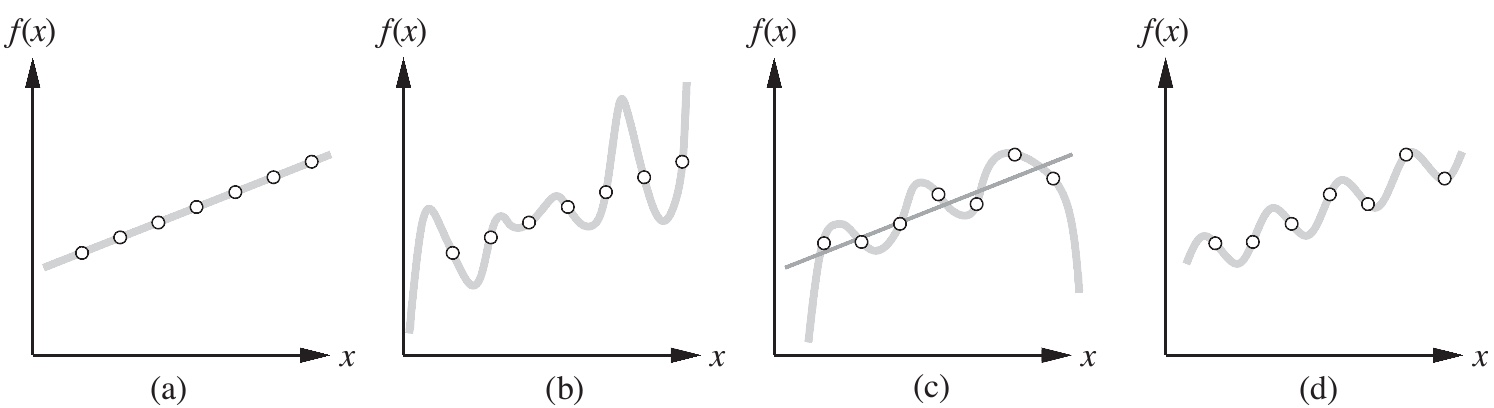
\includegraphics[scale=0.2]{function.jpg}
\caption{(a) linear hypothesis. (b) degree-7 polynomial hypothesis for the same data. (c) regression (approximate linear fit). (d) sinusoidal fit to the same data set.
\label{fig:mission}}
\end{figure}

A classifier is a function that maps an unlabelled instance to a label using internal structures. The output is a set of expected labels for all instances in test set.
Estimating the accuracy of a classifier (agent function) induced by supervised (semi-supervised) learning algorithms is important not only to predict its future prediction accuracy, but also for choosing a classifier from a given set (model selection), or combining classifier (Wolpert 1992).
Based on available data, there are two possible philosophies,\textit{inductive learning} or \textit{transductive learning}.

Induction, in the context of learning, is the attempted discovery of patterns based on the analysis of collected data. The main characteristic of inductive learning is the building of a model – those rules/properties you induce from the data to answer your questions (statistical inference).

Transduction, in the context of learning, refers to reasoning from specific observed (training) instances, to specific observed (unlabelled) instances. It is important to note that not all semi-supervised learning methods are transductive in nature. The main characteristic is the avoidance of building a general model. The information we learn cannot be used to label new instances (which did not have during training). Transductive learning is highly sensitive to noise samples. In my proejct since the embeddings are learned based on the graph structure, the implemented method is transductive, which means we can only predict instances that are already observed in the graph at training time. However, it may be desiderable to have an inductive approach, where generalization hypothesis can be used to predict unseen instances.
%https://codesachin.wordpress.com/2016/07/03/a-small-and-easy-introduction-to-transductive-learning/

\subparagraph{Inductive biases}
Learning is the process of apprehending useful knowledge by observing and interacting with the
world. It involves searching a space of solutions for one expected to provide a better explanation
of the data or to achieve higher rewards. But in many cases, there are multiple solutions which
are equally good (Goodman, 1955). An inductive bias allows a learning algorithm to prioritize
one solution (or interpretation) over another, independent of the observed data (Mitchell,
1980). In a Bayesian model, inductive biases are typically expressed through the choice and
parameterization of the prior distribution (Griffiths et al., 2010). In other contexts, an inductive
bias might be a regularization term (McClelland, 1994) added to avoid overfitting, or it might
be encoded in the architecture of the algorithm itself. Inductive biases often trade flexibility
for improved sample complexity and can be understood in terms of the bias-variance tradeoff
(Geman et al., 1992). Ideally, inductive biases both improve the search for solutions without
substantially diminishing performance, as well as help find solutions which generalize in a
desirable way; however, mismatched inductive biases can also lead to suboptimal performance
by introducing constraints that are too strong.\cite{ind_BIAS}

\section{Graph Neural Network}
%https://arxiv.org/pdf/1806.01261.pdf
According to the explosion of social networks and Big Data, neural networks on graph have been developed and studied  for more than ten years under the umbrella of "graph neural network", but have grown rapdly in the last years.
Here we use \textit{graph} to mean a directed and weighted graph. In the common terminology, a graph is defined as a 2-tuple $G = ( V, A)$. The $V = \{v_i\}_{i=1:N^v}$ is the set of nodes (cardinality $N^v$), where each $v_i$ is a node attribute. The $E = \{(e_k,r_k,s_k)\}_{k=1:N^e}$ is the set of edges (of cardinality $N^e$), where each $e_k$ is the edge's attribute, $r_k$ is the index of the receiver node, and $s_k$ is the index of the sender node. We can easily extend the case of undirected or not-weighted graph.
In data science we can exploit graph properties via the spectral graph theory. The spectral graph theory studies the properties of graph via the eingenvalues and eigenvectors of their associated graph matrices: A (adjacency matrix) and graph Laplacian matrix).
One of the most difficult task for machine learning task is to develop appropriate representations for complex data like graph environment. 
In my project, I consider the problem of constructing a representation for data lying on a high-dimensional space Bag-of-Words \footnote{Bag of Words: The bag-of-words model is a way of representing text data when modeling text with machine learning algorithms. Predominantly bag-of-words model is used in NLP (natural language processing) for document classification. BoW is a way of extracting features from text for use in modeling, but has different drawbacks. It suffers from some shortcomings, such as poor design of vocabulary, sparse representation of space.} model and low-dimensional space with node embedding. Graph are commonly used to encode structural information as protein structure\footnote{Protein structure prediction: is the inference of three-dimensional structure of a protein from its amino acid sequence. The aim of reasercher has been looking at the problem of protein structure matching}.
\subparagraph{Simple Graph}
A simple graph $\mathcal{G}=\{\mathcal{V}, \mathcal{E}\}$ is an undirected graph with neither multiple edges nor loops.
\begin{itemize}
\item $\mathcal{V}(\mathcal{G})= \{v_i,...,v_n\}$ is called the vertex set with n = $|\mathcal{V}|$
\item $\mathcal{E}(\mathcal{G})\subseteq \mathcal{V} \times \mathcal{V}$ is called the vertex set with m = $|\mathcal{E}|$
\item The number of neighbors of a node v is called the degree of v
\item A graph is complete if there is an edge between every pair of
vertices.
\end{itemize}
A graph is called \textit{k-partite} if its set of vertices admits a partiotions into k classes such that the vertitces of the same class are not adjacent.
For simplicity I assume real-valued functions on the set of the graph’s
vertices, $f : V \Rightarrow R$. Such a function assigns a real number
to each graph node. In my project the function f restores a list of features for each node.

\subparagraph{Adjacency Matrix} For a graph with n vertices, the adjacency matrix is defined by $n \times n$ and:
\begin{equation}
A := \begin{cases}
A_{ij} = 1 & \text{if there is an edge $e_{ij}$}\\
A_{ij} = 0 & \text{if there is not an edge}\\
A_{ii} = 0 
\end{cases}
\end{equation}
A is a real-symmetric matrix with n real eingenvalues and its n real eigenvectors form an orthonormal basis.
The adjacency matrix can be viewed as an operator:
\[ g = Af;g(i) = \sum_{e_{ij}} f(j) \]
It can be viewed also as a quadratic form:
$f^T A f =  \sum_{e_{ij}} f(i)f(j) $\\
The connection between the Laplacian and the adjacency matrices:
 $L = D - A$

\subparagraph{Laplacian Matrix}
In the mathematical field of graph theory, the Laplacian matrix, sometimes called admittance matrix, Kirchhoff matrix or discrete Laplacian, is a matrix representation of a graph. The Laplacian matrix can be used to find many useful properties of a graph.

Given a simple graph G with n vertices, its Laplacian matrix $L_{n\times n} $ is defined as: $ L = D-A$ 
where D is the degree matrix and A is the adjacency matrix of the graph. Since \textit{G} is a simple graph, \textit{A} only contains 1s or 0s and its diagonal elements are all 0s.

In the case of directed graphs, either the indegree or outdegree might be used, depending on the application.

The elements of $L$ are given by:

v

The symmetric normalized Laplacian matrix is defined as:
\[
L^{sym} = D^{-\tfrac{1}{2}} L D^{-\tfrac{1}{2}} = I -D^{-\tfrac{1}{2}} A D^{-\tfrac{1}{2}} \] 

The elements $L^{sym}$ are given by:
\begin{equation}
L^{sym}_{i,j}= 
\begin{cases}
1 & \text{if $i=j$ and deg$(v_i) \neq 0$}\\
-\tfrac{1}{\sqrt{deg(v_i)deg(v_j)}} &\text{if $i \neq j$ and $v_i$ is adjacent to $v_j$}\\
0 &\text{otherwise}\\
\end{cases}
\end{equation}
\begin{figure}[htbp]
\centering
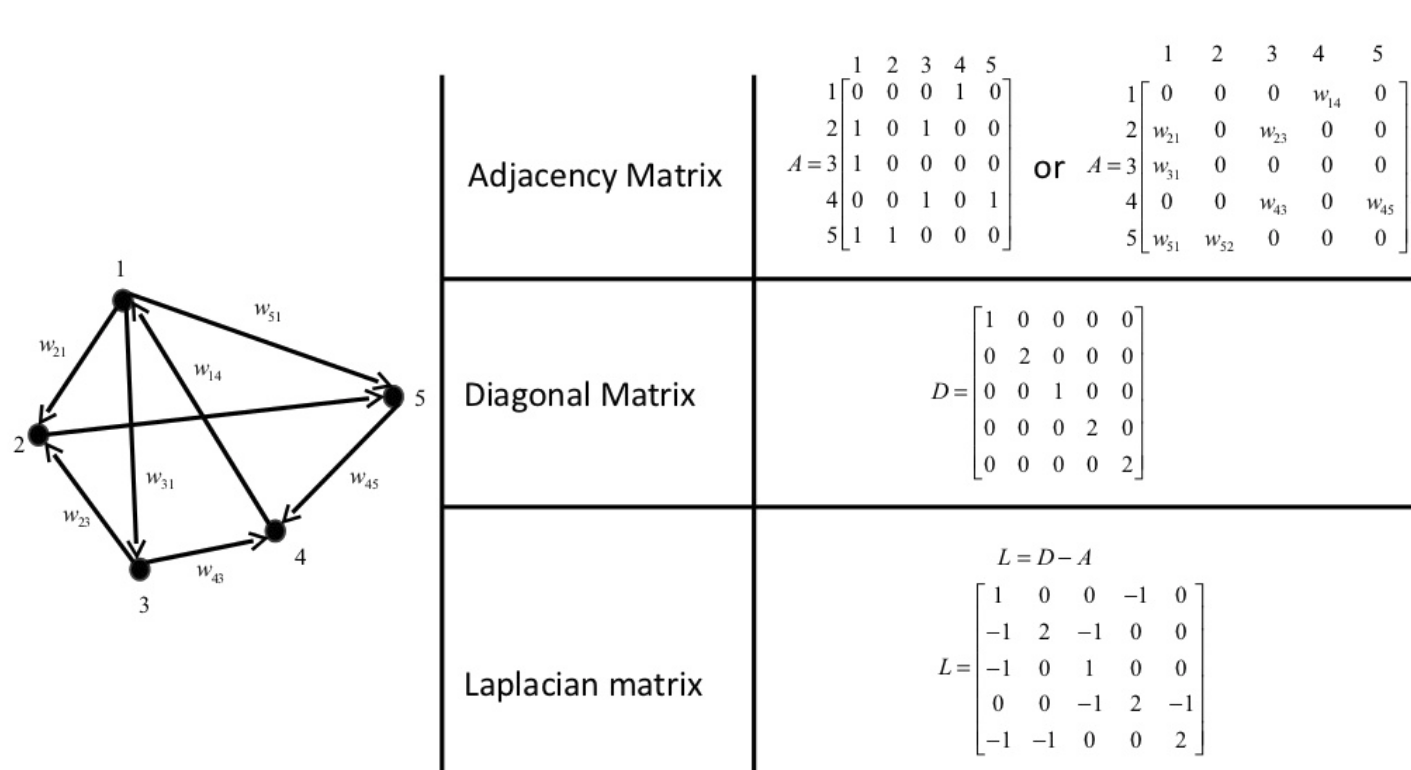
\includegraphics[scale=0.2]{res_ALD2.png}
\caption{ Recap of graph matrices
\label{fig:map}}
\end{figure}
%fa cagare l'immagine
The Laplacian allows to link between discrete representations (e.g graph, linked structures) and continuous representation (e.g vector space)\footnote{For example we can map a graph on a line such that connected nodes stay as close as possible (i.e arg min$(f^T L f )$ with $f^Tf=1$)}.
We can see Laplacian as an operator in simple graph weighted as:
\[ f^T L f = \dfrac{1}{2}\sum_{e_{ij}} w_{ij}|f(v_i)-f(v_j)|^2    \text{            	with $w_{ij}>0$} \] 

\begin{figure}[htbp]
\centering
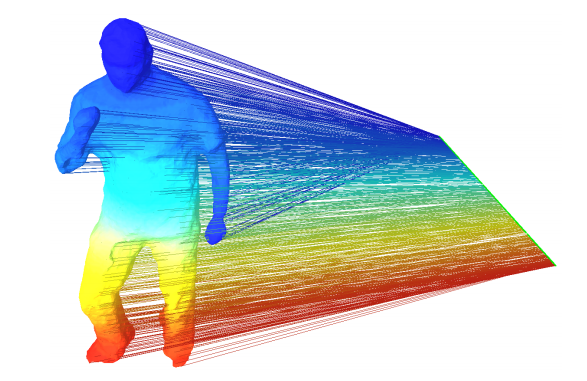
\includegraphics[scale=0.25]{map.png}
\caption{ Example of mapping a graph on the Fiedler vector
\label{fig:map}}
\end{figure}

\subparagraph{Graph Partitionning Problem}
The main application of laplacian is spectral clustering that corresponds to a computationally performant solution to the graph partitionning problem \\
Given: 
$G = (V, E) $ and  P number of partitions.\\ Output:
	Compute a (vertex) partition $V=V_0 \cup V_1 \cup ... V_{p-1}$ such that:
	\begin{enumerate}
	\item $ \{V_i \} $ are disjoint $\Rightarrow V_i \cap V_j = \oslash$
	\item $ \{V_i \} $ are roughly balanced $\Rightarrow |V_i| \approx |V_j| $
	\item let $E_{cut} \equiv \{ (u,v) | u \in V_i, v \in V_j, i \neq j\} $ :  minimize $E_{cut}$
	\end{enumerate}


\subsection{Learning Architectures}
%https://arxiv.org/pdf/1806.01973.pdf
Most prominent among these advancements is the success
of deep learning architectures known as Graph Convolutional
Networks (GCNs). The core idea behind GCNs is
to learn how to iteratively aggregate feature information from local
graph neighborhoods using neural networks. Here a
single “convolution” operation transforms and aggregates feature
information from a node’s one-hop graph neighborhood, and by
stacking multiple such convolutions information can be propagated
across far reaches of a graph (figure \ref{fig:conv}). Unlike purely content-based deep
models (e.g., recurrent neural networks), GCNs leverage both
content information as well as graph structure. 
The main challenge is to correctly size and find the right combination of both the BoW as well as node embeddings.\cite{deep_GCN}.


\begin{figure}[htbp]
\centering
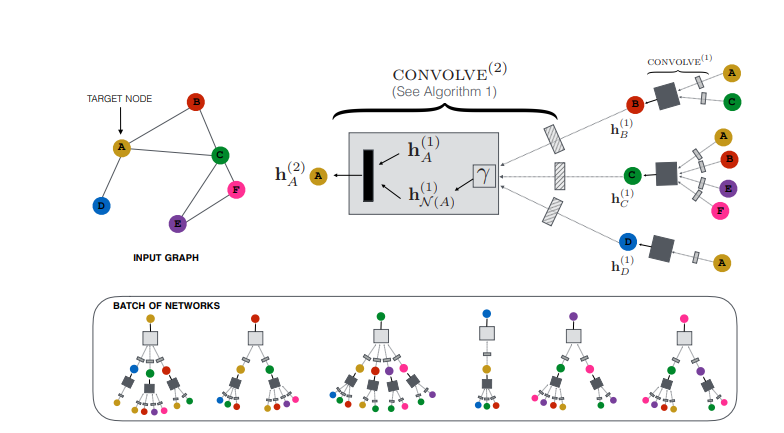
\includegraphics[scale=0.4]{gconv.png}
\caption{Graph using depth-2 convolution}
\label{fig:conv}
\end{figure}


\section{Related Work}
In this project we consider the problem of classifying nodes (such as scientific documents) in a directed graph,  where the labels are only available for a small subset of nodes. This problem can be framed as graph-based semi-supervised learning. \cite{Kipf_GCN}. Given a network of citations and a reduced amount of labels, the agent try to predict node label from its knowledge base.


\section{State of the Art}
In this section I present the state of the art regarding the main technologies used in the project.
First of all I contextualize on neural networks.
\subsection{Object Classification Problem}
In this problem we have a set of objects, which can be document and we may suppose that the numerical representation of an object is a n-dimensional vector $x \in R$. There exists a function $f : R^n \rightarrow {1, 2, . . . , K}$, that associate to each object x a class $f(x)$, where $K \in \mathbb{N}$ (also known as label), is the number of different classes (e.g. x is an image and f(x)
is the subject of the image). The solution to the classification problem consists in
determining a function equivalent to f (also known as hypothesis).
The classification problem can also be related to other tasks such as node detection in graph.

The output of the NN, is a highly complex non-linear function $z(x) \in \mathbb{R}^K$,
which, in turn, is dependent on the parameters of the NN. This function is used to obtain a probability distribution of the class $j$ given the object $x$, called the
\textit{softmax function}. If $z_j(x)$ is the j-th component of $z(x)$, j = 1, . . . , K then the softmax function is given by:
\[
p(j|x) = \dfrac{e^{z_j(x)}}{\sum_{i=1}^{K} e^{z_i(x)}}
\]
The goal is to obtain a softmax function such taht $f(x)=argmax_jp(j|x)$.
In order to do this a NN is trained using a training set D. Each element of D is a couple $(x_i,f(x_i)), i=1,2,...,N$ and N is the size of the training set. In order to determine the accuracy of the network, a loss function is employed, that assigns to each object x a quantitative measure of the error the NN made in
classifying x. Often, the loss function takes the negative logarithm of the softmax function as follows
\[
L(x)=-log\ p(f(x)|x)
\]
and, in order to improve the NN, the gradients (with respect to the parameters of the NN, hidden in the definition of z) of the mean of the loss function over all training set
\[
L = -\dfrac{1}{N}\sum_{i=1}^{N} log\ p(f(x_i)|x_i) 
\]
are back propagated along all the layers of the NN. The negative logarithm of the softmax function can be interpreted as the \textit{cross-entropy} between the probability
distribution given in softmax function and the true probability $q(j|x)$ of the class $j$ given the object $x$.

\[
\mathbb{H}(q,p) = - \sum_{i=1}^{K} q(i|x) log\ p(i|x) 
\]
In most of the literature regarding the cross-entropy loss function in NN, the
probability distribution q is taken as follows
\begin{equation}
q(j|x)= 
\begin{cases}
1 & \text{if $f(x)=j$ }\\
0 &\text{otherwise}\\
\end{cases}
\end{equation}
and having chose q as above, and substituting it in $\mathbb{H}$, one obtains \\ $L(x)=-log\ p(f(x)|x)$  which
is commonly referred to as the categorical cross-entropy.

One of the main problem in training a neural network is the over-fitting. The
over-fitting of a neural network, is the problem that prevent the network to generalize
and obtain accurate prediction on samples not contained in the training set. Moreover and worse, one finds that, sometimes, the training process spends a
lot of time to reduce the loss without even achieve better fitting on the training
set. With a close inspection in fact one can observe that a considerable amount
of the time is spent, by the training process, on Loss function to make better an already good and accurate prediction.

\subsection{Graph Convolutional Neural Networks}
%https://towardsdatascience.com/how-to-do-deep-learning-on-graphs-with-graph-convolutional-networks-7d2250723780
%https://tkipf.github.io/graph-convolutional-networks/
Today, graph convolutional neural networks are a powerful neural network architecture for machine learning on graphs. In fact, they are so powerful that even a randomly initiated 2-layer GCN can produce useful feature representations of nodes in networks. 
More formally, a graph convolutional network (GCN) is a neural network that operates on graphs. Given a graph, a GCN takes as input:
\begin{itemize}
\item an input feature matrix $N \times F^0$, feature matrix X, where N is the number of nodes and $F^0$ is the number of input features for each node.
\item an $N \times N$ matrix representation of the graph structure such as the adjacency matrix A of G.

\end{itemize}

A hidden layer in the GCN can thus be written as $H^i = f(H^{i-1},A)$ where $H^0 = X$ and f is the propagation function. Each layer $H^i$ corresponds to an $N \times F^i$ feature matrix where each row is a feature representation of a node. At each layer, these features are aggregated to form the next layer’s features using the propagation rule \textit{f}. In this way, features become increasingly more abstract at each consecutive layer. In this framework, variants of GCN differ only in the choice of propagation rule f.

In our case X is a matrix (bag of words features) and A is the adiacency matrix of the graph.
%https://arxiv.org/pdf/1806.01973.pdf



\subsection{Semi-supervised Node Classification}
%https://arxiv.org/pdf/1609.02907.pdf
%https://arxiv.org/pdf/1603.08861.pdf
\subsection{Node Embedding}
%https://csustan.csustan.edu/~tom/Clustering/GraphLaplacian-tutorial.pdf
%https://arxiv.org/pdf/1607.00653.pdf
\subsection{K-fold Cross Validation}
%https://www.researchgate.net/profile/Ron_Kohavi/publication/2352264_A_Study_of_Cross-%Validation_and_Bootstrap_for_Accuracy_Estimation_and_Model_Selection/links/02e7e51bcc14c5e91c000000.pdf

\section{Method}
\subsection{Problem Setup}
Here we present ...
The embedding of an instance is
jointly trained to predict the class label of the instance and
the context in the graph. We then concatenate the embeddings
and the hidden layers of the original classifier and
feed them to a softmax layer when making the prediction.
\subsection{Node Embeddings via Node2Vec}
%https://arxiv.org/pdf/1607.00653.pdf
\section{Experiments and Results}

\subsection{Dataset}
Cora
\subsection{Experimental Set-Up}

\section{Conclusion}

Lorem ipsum dolor sit amet, consectetur adipisicing elit, sed do eiusmod tempor
incididunt ut labore et dolore magna aliqua. Ut enim ad minim veniam, quis
nostrud exercitation ullamco laboris nisi ut aliquip ex ea commodo consequat.
Duis aute irure dolor in reprehenderit in voluptate velit esse cillum dolore eu
fugiat nulla pariatur.

\bibliographystyle{plain}

\bibliography{mybib}

\end{document}
